\documentclass[tikz,border=2pt]{standalone}
\usepackage{newpxtext,newpxmath}
\definecolor{curve}{HTML}{1f6fb2}
\definecolor{accent}{HTML}{c0392b}
\definecolor{polygon}{HTML}{555555}
\definecolor{muted}{HTML}{dfe6ee}
\begin{document}
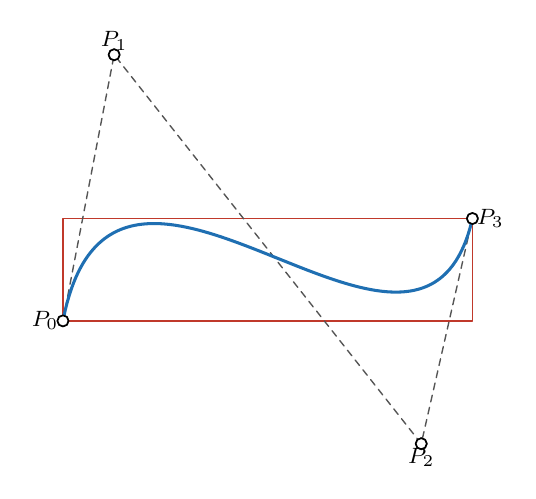
\begin{tikzpicture}[
  x=1.3cm, y=1.3cm,
  line cap=round, line join=round,
  every node/.style={font=\footnotesize, inner sep=1.5pt},
  curve/.style={draw=curve, line width=1.1pt},
  second/.style={draw=accent, line width=1.1pt},
  polygon/.style={line width=0.5pt, dash pattern=on 2.5pt off 2pt},
  construction/.style={draw=accent, line width=0.5pt},
  axis/.style={line width=0.45pt, draw=black!80, >=stealth},
  ctrl/.style={circle, fill=white, line width=0.6pt, minimum size=4pt, inner sep=0pt},
]
\draw[accent, line width=0.6pt] (0,0) rectangle (4,1);
\draw[polygon, draw=polygon] (0,0) -- (0.5,2.6) -- (3.5,-1.2) -- (4,1);
\node[ctrl, draw=polygon] at (0,0) {};
\node[ctrl, draw=polygon] at (0.5,2.6) {};
\node[ctrl, draw=polygon] at (3.5,-1.2) {};
\node[ctrl, draw=polygon] at (4,1) {};
\node[left] at (0,0) {$P_0$};
\node[above] at (0.5,2.6) {$P_1$};
\node[below] at (3.5,-1.2) {$P_2$};
\node[right] at (4,1) {$P_3$};
\draw[curve] (0.0000,0.0000) .. controls (0.5000,2.6000) and (3.5000,-1.2000) .. (4.0000,1.0000);
\node[ctrl, draw=black] at (0,0) {};
\node[ctrl, draw=black] at (0.5,2.6) {};
\node[ctrl, draw=black] at (3.5,-1.2) {};
\node[ctrl, draw=black] at (4,1) {};
\end{tikzpicture}
\end{document}
